




\clearpage
\newpage
\section{\textsc{GRACE}: \underline{G}eometric \underline{R}epresentation-\underline{A}ware \underline{C}ontrastive \underline{E}nhancement}

While Direct Preference Optimization (DPO)~\cite{rafailov2023direct} has emerged as a compelling paradigm for aligning language models with human preferences, it primarily operates at the output logit level—optimizing models to prefer safe completions over unsafe ones. However, adversarial attacks do not merely exploit generation probabilities; they camouflage unsafe intent within benign-looking prompts that remain indistinguishable in the model’s internal representation space. In such cases, alignment must extend beyond the surface form to actively reshape the geometry of latent activations.

We propose \textsc{GRACE}—a novel alignment framework that augments preference-based objectives with \textit{representation-level contrastive regularization}. Inspired by Generalized DPO (GRPO)~\cite{wu2024generalized}, \textsc{GRACE} modifies the DPO objective to enforce stronger separation in the model’s hidden space between safe and adversarial completions. By imposing latent contrast and relaxing the KL constraint, \textsc{GRACE} not only preserves preference-consistent outputs but also carves out distinct topological subspaces for safe and unsafe behaviors.









\section{\textsc{GRACE}: Geometric Representation-Aware Contrastive Enhancement}

Motivated by this hypothesis, we introduce \textsc{GRACE}, a principled extension of DPO that injects structural inductive bias into the alignment process. Specifically, \textsc{GRACE} augments preference optimization with two geometric components:

\begin{enumerate}
    \item \textbf{Geometric Separation Constraint.} We introduce a regularization term that enforces linear separability between safe, unsafe, and jailbreak completions in hidden space—explicitly maximizing centroid distance and minimizing overlap.
    
    \item \textbf{Latent Contrastive Enhancement.} We incorporate a contrastive loss that sharpens intra-cluster cohesion among safe generations while pushing unsafe completions toward isolated subspaces. This regularization is applied across multiple layers to ensure robust representational separation.
\end{enumerate}

Together, these modifications reframe alignment as a dual optimization problem: learning which outputs to prefer and how to encode those preferences into the model’s latent manifold. As our experiments show, \textsc{GRACE} transforms adversarial vulnerability into a problem of geometric insulation—shielding safe behavior from manipulation by reshaping the structure of thought itself.





\subsection{Desired Geometric Structure for Robust Adversarial Alignment}

To probe internal behaviors of aligned language models under adversarial attack, we apply our Adversarial Vulnerability Quality Index (AVQI) and perform cluster-level analysis across hidden layers. This reveals the following consistent structure:

\begin{enumerate}
    \item \textbf{Safe completions form compact, low-variance clusters} in latent space, suggesting a well-regularized internal encoding of benign behavior.

    \item \textbf{Adversarial generations tend to lie deceptively close to safe completions}, often near the boundary of the safe region. This induces a \emph{camouflage effect}, where adversarial responses become representationally similar to safe ones, eluding standard alignment signals.

    \item \textbf{Ideal structure:} Robust alignment requires \emph{orthogonal separation} between safe and unsafe/adversarial behaviors. Despite differing attack modalities, unsafe and adversarial completions should coalesce into a coherent adversarial subspace.
\end{enumerate}

These findings expose a key limitation of preference-only optimization (e.g., DPO): while it enforces surface-level output behavior, it fails to impose the internal geometric structure necessary for generalization to obfuscated or unseen attacks.

To address this, we introduce a latent-space regularization objective that explicitly encourages:
\begin{itemize}[nosep,leftmargin=1em]
    \item separation of safe from adversarial representations,
    \item and consolidation of unsafe and jailbreak generations into a unified adversarial manifold.
\end{itemize}

Embedding such geometric priors during training enables the model to internalize behavioral semantics, fostering both interpretability and robustness under adversarial perturbations.




\begin{comment}
\begin{figure*}[t]
\centering
\begin{tcolorbox}[
  enhanced,
  colback=white,
  colframe=black,
  boxrule=1pt,
  borderline={0.6pt}{2pt}{black},
  sharp corners,
  width=\textwidth,
]
\vspace{-4mm}
\[
\begin{aligned}
\min_{\theta} \quad & 
\underbrace{-\log \sigma\Big(
\log \pi_\theta(y_{\mathrm{safe}} \mid x)
- \log \pi_\theta(y_{\mathrm{adv}} \mid x)
- \alpha \left[
\log \pi_{\mathrm{ref}}(y_{\mathrm{safe}} \mid x)
- \log \pi_{\mathrm{ref}}(y_{\mathrm{adv}} \mid x)
\right]
\Big)}_{\text{(1) Relaxed Preference Loss}}
\\[6pt]
& +\; \lambda \Big[
\underbrace{
\sum_{\substack{h_s \in C_{\mathrm{safe}} \\ h_a \in C_{\mathrm{adv}}}} 
\max(0,\; M - \|h_s - h_a\|_2)
}_{\text{(2) Safe--Adversarial Separation}}
\;+\;
\underbrace{
\sum_{\substack{h_u \in C_{\mathrm{unsafe}} \\ h_j \in C_{\mathrm{jb}}}} 
\max(0,\; \|h_u - h_j\|_2 - \delta)
}_{\text{(3) Unsafe--Jailbreak Merging}}
\Big]
\end{aligned}
\]
\vspace{-4mm}
\end{tcolorbox}

\vspace{-2mm}
\caption{
\textbf{Final Objective for Geometric Preference Optimization.} The total loss balances preference alignment and geometric regularization:
\begin{itemize}[noitemsep,leftmargin=1em]
    \item \textbf{(1) Relaxed Preference Loss:} Softens the KL constraint via $\alpha$ while ensuring $y_{\mathrm{safe}}$ is preferred over $y_{\mathrm{adv}}$.
    \item \textbf{(2) Safe--Adversarial Separation:} Pushes latent representations of safe and adversarial generations apart by a margin $M$.
    \item \textbf{(3) Unsafe--Jailbreak Merging:} Encourages unsafe and jailbreak responses to form a compact adversarial cluster within distance $\delta$.
\end{itemize}
Hyperparameters $\lambda$, $\alpha$, $M$, and $\delta$ jointly govern the preference-geometric balance for improved adversarial robustness.
}
\label{fig:final_objective_geometric_dpo}
\vspace{-2mm}
\end{figure*}
\end{comment}


\subsection{Latent Geometric Regularization Loss}

Motivated by the observed geometric patterns in hidden representations, we introduce a latent-space regularization objective that promotes the desired separation between behavioral classes. Our goal is twofold: (1) to enforce representational separation between safe and adversarial completions, and (2) to consolidate unsafe and jailbreak generations into a coherent adversarial subspace.

Let $h_\theta(x, y)$ denote the hidden representation of a prompt–response pair, extracted from a designated intermediate layer. We define the following sets:
\[
C_{\mathrm{safe}},\quad C_{\mathrm{unsafe}},\quad C_{\mathrm{jb}} \subset \mathbb{R}^d
\]
representing latent vectors corresponding to safe, unsafe, and jailbreak completions, respectively.

Inspired by supervised contrastive learning~\cite{khosla2020supervised} and metric learning via triplet loss~\cite{schroff2015facenet}, we define two margin-based constraints:

\vspace{1mm}
\textbf{(1) Safe–Adversarial Separation.} To increase separation between safe and adversarial representations (including both unsafe and jailbreak), we define a contrastive loss:
\[
\mathcal{L}_{\mathrm{sep}} = \sum_{\substack{h_s \in C_{\mathrm{safe}} \\ h_a \in C_{\mathrm{adv}}}} \max(0,\; M - \|h_s - h_a\|_2)
\]
where $C_{\mathrm{adv}} = C_{\mathrm{unsafe}} \cup C_{\mathrm{jb}}$ and $M$ is a minimum separation margin.

\vspace{1mm}
\textbf{(2) Unsafe–Jailbreak Consolidation.} To encourage geometric similarity between unsafe and jailbreak clusters, we introduce a proximity constraint:
\[
\mathcal{L}_{\mathrm{merge}} = \sum_{\substack{h_u \in C_{\mathrm{unsafe}} \\ h_j \in C_{\mathrm{jb}}}} \max(0,\; \|h_u - h_j\|_2 - \delta)
\]
where $\delta$ defines the maximum allowable spread within the adversarial subspace.





\vspace{1mm}
\subsection{Final Loss: Preference-Guided Geometric Optimization}

To complete the training loss, we combine the relaxed preference optimization objective with our latent cluster regularization terms. This joint objective balances behavioral alignment at the output level with geometric consistency in the hidden representation space:
\[
\mathcal{L}_{\text{total}} = \mathcal{L}_{\text{pref}} + \lambda_{\text{sep}}\, \mathcal{L}_{\mathrm{sep}} + \lambda_{\text{merge}}\, \mathcal{L}_{\mathrm{merge}}
\]
Here, $\mathcal{L}_{\text{pref}}$ represents the primary preference optimization term, which encourages the model to assign higher likelihood to safe completions over adversarial ones. The auxiliary terms, $\mathcal{L}_{\mathrm{sep}}$ and $\mathcal{L}_{\mathrm{merge}}$, impose geometric constraints on the model's latent space. Specifically, $\mathcal{L}_{\mathrm{sep}}$ increases the representational distance between safe and adversarial examples, while $\mathcal{L}_{\mathrm{merge}}$ encourages unsafe and jailbreak generations to occupy a shared adversarial subspace. The corresponding weights $\lambda_{\text{sep}}$ and $\lambda_{\text{merge}}$ balance the influence of these geometric regularizers relative to the main alignment objective.

This composite loss guides the model to:
\begin{itemize}[nosep,leftmargin=1.5em]
    \item Align with preference annotations by preferring safe responses over adversarial ones ($\mathcal{L}_{\text{pref}}$),
    \item Create latent separation between safe and adversarial behaviors ($\mathcal{L}_{\mathrm{sep}}$),
    \item Geometrically unify unsafe and jailbreak completions into a compact adversarial cluster ($\mathcal{L}_{\mathrm{merge}}$).
\end{itemize}

This objective integrates output-level supervision with latent-space structuring, fostering alignment in the model’s predictions and the internal representation space, enabling more generalizable and mechanistically grounded adversarial robustness.










\subsection{Expanded Final Loss with Learned Pooled Representations}

The structure of the total alignment loss remains unchanged:
\[
\mathcal{L}_{\mathrm{total}} = \mathcal{L}_{\mathrm{pref}} + \lambda_{\mathrm{sep}} \cdot \mathcal{L}_{\mathrm{sep}} + \lambda_{\mathrm{merge}} \cdot \mathcal{L}_{\mathrm{merge}}
\]
However, the internal computation of $\mathcal{L}_{\mathrm{sep}}$ and $\mathcal{L}_{\mathrm{merge}}$ is transformed by the learned attention profile $\alpha^{(l)}$.

\vspace{1mm}
\noindent\textbf{Old setting (before attention pooling):} Representations were extracted only from the final layer:
\[
\tilde{h}_y = h_y^{(L)}
\]

\vspace{1mm}
\noindent\textbf{New setting (after attention pooling):} Representations are computed as a weighted sum across layers:
\[
\tilde{h}_y = \sum_{l=1}^{L} \alpha^{(l)} h_y^{(l)}, \quad \text{where } \sum_l \alpha^{(l)} = 1,\; \alpha^{(l)} \geq 0
\]

This change impacts both latent terms in the loss.

\vspace{1mm}
\noindent\textbf{Expanded $\mathcal{L}_{\mathrm{sep}}$:}
\[
\begin{aligned}
\mathcal{L}_{\mathrm{sep}} &=
\max\left(0,\; M - \left\| \sum_{l=1}^L \alpha^{(l)} \left( h^{(l)}_{\text{safe}} - h^{(l)}_{\text{unsafe}} \right) \right\|_2 \right) \\
&\quad + \max\left(0,\; M - \left\| \sum_{l=1}^L \alpha^{(l)} \left( h^{(l)}_{\text{safe}} - h^{(l)}_{\text{jb}} \right) \right\|_2 \right)
\end{aligned}
\]

\vspace{1mm}
\noindent\textbf{Expanded $\mathcal{L}_{\mathrm{merge}}$:}
\[
\mathcal{L}_{\mathrm{merge}} =
\max\left(0,\; \left\| \sum_{l=1}^L \alpha^{(l)} \left( h^{(l)}_{\text{unsafe}} - h^{(l)}_{\text{jb}} \right) \right\|_2 - \delta \right)
\]

This formulation shows how $\alpha^{(l)}$ actively controls the distance computation across layers — creating a soft projection of geometric behavior that blends semantic signals from multiple layers.

\vspace{1mm}
\noindent\textbf{Gradient Flow.}
If $\alpha$ is treated as trainable, gradients from $\mathcal{L}_{\mathrm{sep}}$ and $\mathcal{L}_{\mathrm{merge}}$ flow through the weighted differences:
\[
\nabla_{\alpha^{(l)}} \mathcal{L}_{\mathrm{merge}},\quad \nabla_{\alpha^{(l)}} \mathcal{L}_{\mathrm{sep}} \neq 0
\]

\noindent If $\alpha$ is fixed (pre-trained), these terms are treated as constants during optimization of model parameters.

\vspace{1mm}
\noindent\textbf{Impact.} \\
By replacing static single-layer representations with weighted layerwise combinations, this updated loss:
\begin{itemize}[leftmargin=1.5em]
    \item Induces richer geometry across behavior types (safe, unsafe, jailbreak).
    \item Avoids overfitting to a specific depth (e.g., last layer).
    \item Enables generalization via attention-tuned latent spaces.
\end{itemize}

\subsection{Relaxing KL Constraints: From DPO to GRPO}

Direct Preference Optimization (DPO)~\cite{rafailov2023direct} optimizes a pairwise logistic preference loss, with a KL-like term that constrains divergence from a reference model:
\[
\mathcal{L}_{\mathrm{DPO}} = -\log \sigma\left(
\log \pi_\theta(y_{\mathrm{safe}} \mid x) -
\log \pi_\theta(y_{\mathrm{unsafe}} \mid x) -
\Delta_{\mathrm{ref}}
\right)
\]
where
\[
\Delta_{\mathrm{ref}} =
\log \pi_{\mathrm{ref}}(y_{\mathrm{safe}} \mid x) -
\log \pi_{\mathrm{ref}}(y_{\mathrm{unsafe}} \mid x)
\]

This reference term acts as a surrogate for the reverse KL between the learned policy $\pi_\theta$ and the reference policy $\pi_{\mathrm{ref}}$, and helps stabilize training by preventing undesirable mode collapse. However, it also limits flexibility—especially when the reference model itself may be poorly calibrated or unsafe under adversarial conditions.

\vspace{1mm}
\textbf{From KL Constraints to Controlled Drift.} \\
Inspired by recent advances such as GRPO~\cite{wu2024generalized} and $\varepsilon$-DPO~\cite{chen2023epsilon}, we propose a relaxed version of the preference loss that introduces an adjustable scale $\alpha \in [0,1]$:
\[
\mathcal{L}_{\mathrm{pref}} = -\log \sigma\left(
\log \pi_\theta(y_{\mathrm{safe}} \mid x) -
\log \pi_\theta(y_{\mathrm{adv}} \mid x) -
\alpha \Delta_{\mathrm{ref}}
\right)
\]

Here, $\alpha$ governs the strength of the KL regularization. When $\alpha = 1$, we recover standard DPO. When $\alpha = 0$, the loss becomes fully reference-free, letting the model optimize preferences without constraint. This relaxation allows the policy to learn safer completions even when the reference model fails to differentiate between benign and adversarial outputs.

\vspace{1mm}
\textbf{Toward Structured Alignment.} \\
While $\mathcal{L}_{\mathrm{pref}}$ guides behavioral preference at the output level, it lacks any structural incentive for how safe and adversarial examples should be represented internally. To address this, we incorporate latent-space supervision via our learned pooled representations $\tilde{h}_y = \sum_l \alpha^{(l)} h_y^{(l)}$.

The full training objective becomes:
\[
\mathcal{L}_{\mathrm{total}} =
\mathcal{L}_{\mathrm{pref}} +
\lambda_{\mathrm{sep}} \cdot \mathcal{L}_{\mathrm{sep}} +
\lambda_{\mathrm{merge}} \cdot \mathcal{L}_{\mathrm{merge}}
\]

Here:
\begin{itemize}[leftmargin=1.5em]
    \item $\mathcal{L}_{\mathrm{pref}}$ is the relaxed DPO loss above,
    \item $\mathcal{L}_{\mathrm{sep}}$ encourages geometric separation of safe vs. adversarial completions, and
    \item $\mathcal{L}_{\mathrm{merge}}$ ensures unsafe and jailbreak examples reside in a unified adversarial subspace.
\end{itemize}

This formulation allows preference alignment and latent geometry to be learned in tandem, while avoiding over-reliance on an imperfect reference policy.



\begin{figure*}[t]
    \centering
    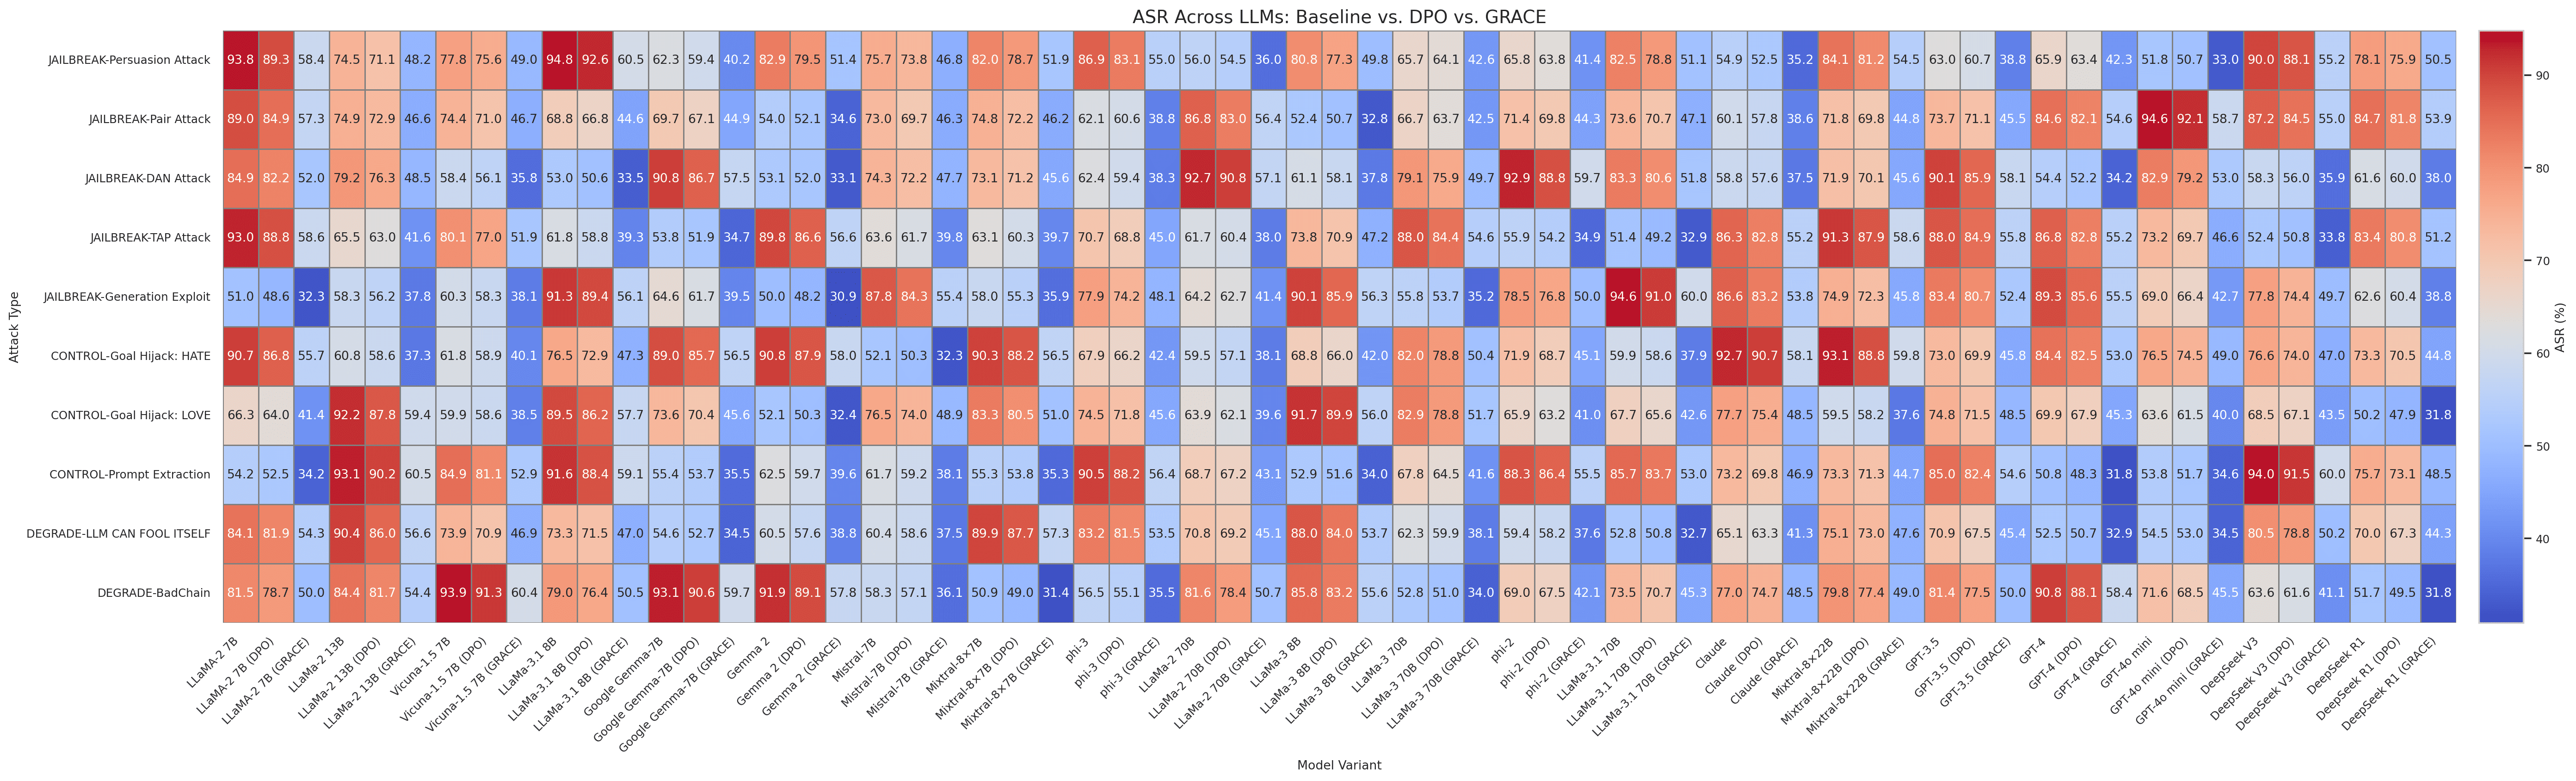
\includegraphics[width=\textwidth]{figures/results.png}
    \caption{
    \textbf{Adversarial Robustness Across LLMs: Baseline vs. DPO vs. GRACE}
    This heatmap illustrates Attack Success Rates (ASR, in \%) across various adversarial attacks for 21 popular LLMs under three training configurations: baseline (original model), DPO fine-tuning, and our proposed GRACE fine-tuning. Rows correspond to adversarial attacks grouped into three broad categories: \emph{Jailbreak}, \emph{Control Hijacking}, and \emph{Degradation}. Columns are grouped by model, each with three versions: Baseline, DPO, and GRACE. 
    \textbf{Key observations:} (1) DPO offers modest ASR reduction (2–5\% on average); (2) GRACE significantly reduces ASR (35–39\% reduction); (3) Models like GPT-4 and Mixtral show substantial improvements across high-risk attacks (e.g., DAN, Goal Hijack, and BadChain). The intense color contrast shows that GRACE consistently outperforms DPO in neutralizing adversarial completions while preserving generalization across model scales and families.
    }
    \label{fig:asr_heatmap_grace}
\end{figure*}





\begin{figure*}[t]
\centering
\begin{tcolorbox}[
  enhanced,
  colback=white,
  colframe=black,
  boxrule=1pt,
  borderline={0.6pt}{2pt}{black},
  sharp corners,
  width=\textwidth,
]
\vspace{-4mm}
\[
\begin{aligned}
\min_{\theta} \quad & 
\underbrace{-\log \sigma\left(
\log \pi_\theta(y_{\mathrm{safe}} \mid x)
- \log \pi_\theta(y_{\mathrm{adv}} \mid x)
- \alpha \big[
\log \pi_{\mathrm{ref}}(y_{\mathrm{safe}} \mid x)
- \log \pi_{\mathrm{ref}}(y_{\mathrm{adv}} \mid x)
\big]
\right)}_{\text{(1) Relaxed Preference Loss}} \\[6pt]
& +\; \lambda_{\mathrm{sep}} \cdot
\underbrace{
\left[
\max\left(0,\; M - \left\| \tilde{h}_{\mathrm{safe}} - \tilde{h}_{\mathrm{unsafe}} \right\|_2 \right)
+
\max\left(0,\; M - \left\| \tilde{h}_{\mathrm{safe}} - \tilde{h}_{\mathrm{jb}} \right\|_2 \right)
\right]
}_{\text{(2) Safe--Adversarial Latent Separation}} \\[6pt]
& +\; \lambda_{\mathrm{merge}} \cdot
\underbrace{
\max\left(0,\; \left\| \tilde{h}_{\mathrm{unsafe}} - \tilde{h}_{\mathrm{jb}} \right\|_2 - \delta \right)
}_{\text{(3) Unsafe--Jailbreak Latent Merging}}
\end{aligned}
\]
\vspace{-4mm}
\end{tcolorbox}

\vspace{-2mm}
\caption{
\textbf{Final Objective for Geometric Preference Optimization.} This loss integrates relaxed preference alignment with latent-space regularization using pooled representations $\tilde{h}_y = \sum_l \alpha^{(l)} h_y^{(l)}$:
\begin{itemize}[noitemsep,leftmargin=1em]
    \item \textbf{(1) Relaxed Preference Loss:} Generalizes DPO by introducing a scaling factor $\alpha$ over the reference model KL constraint $\Delta_{\mathrm{ref}}$, improving robustness when $\pi_{\mathrm{ref}}$ is unsafe.
    \item \textbf{(2) Latent Separation:} Encourages margin-based distancing between safe and both unsafe/jailbreak representations using $\tilde{h}_y$.
    \item \textbf{(3) Latent Merging:} Promotes representational cohesion between unsafe and jailbreak examples within a threshold $\delta$.
\end{itemize}
All latent terms operate on frozen LLM representations pooled via $\alpha^{(l)}$, while gradients flow only into the policy $\pi_\theta$ and optionally $\alpha$. Hyperparameters $(\alpha, \lambda_{\mathrm{sep}}, \lambda_{\mathrm{merge}}, M, \delta)$ control the trade-off between behavioral fidelity and latent alignment.
}
\label{fig:final_objective_geometric_dpo}
\vspace{-2mm}
\end{figure*}